\documentclass[10pt]{article}
\usepackage{fullpage}
\usepackage{amsmath,amsfonts,amsthm}
\usepackage{graphicx}
\usepackage{listings}
\usepackage{float}
\graphicspath{ {./figure/} }

\usepackage{enumitem}
\usepackage{amssymb}
\usepackage{amsmath}
\usepackage{fancyvrb}
\usepackage{venndiagram}
\usepackage{tikz}
\newtheorem{example}{Example}
\usepackage{alltt,xcolor}


\newcommand{\redbullet}{$\textcolor{red}{\bullet}$}
\newcommand{\bluebullet}{$\textcolor{blue}{\bullet}$}

\newcommand{\red}[1]{\textcolor{red}#1}
\newcommand{\green}[1]{{\color{green}#1}}
\newcommand{\blue}[1]{{\color{blue}#1}}
\newcommand{\purple}[1]{{\color{purple}#1}}
\newcommand{\orange}[1]{{\color{orange}#1}}
\newcommand{\hashjoin}[1]{\begin{array}{c} \mathtt{hashJoin} \\ \bowtie\\ {#1}\\ \end{array}}
\newcommand{\mergejoin}[1]{\begin{array}{c} \mathtt{mergeJoin} \\ \bowtie\\ {#1}\\ \end{array}}
\newcommand{\indexjoin}[1]{\begin{array}{c} \mathtt{indexJoin} \\ \bowtie\\ {#1}\\ \end{array}}
\newcommand{\nestedjoin}[1]{\begin{array}{c} \mathtt{nestedLoopJoin} \\ \bowtie\\ {#1}\\ \end{array}}

\newcommand{\sortprojection}[1]{\begin{array}{c} \mathtt{sortProjection} \\ \pi_{#1}\ \end{array}}
\newcommand{\hashprojection}[1]{\begin{array}{c} \mathtt{hashProjection} \\ \pi_{#1}\ \end{array}}
\newcommand{\scan}[1]{\begin{array}{c} \mathtt{scan} \\ {#1}\ \end{array}}
\newcommand{\filter}[1]{\begin{array}{c} \mathtt{filterSelection}\\ \sigma_{#1}\ \end{array}}
\newcommand{\filterscan}[2]{\begin{array}{c} \mathtt{filterScan}\\ \sigma_{#1}(#2)\ \end{array}}
\newcommand{\sortfilterscan}[2]{\begin{array}{c}\mathtt{sort} \mathtt{filterScan}\\ \sigma_{#1}(#2)\ \end{array}}



\author{Team 37}
\title{Homework 6 -- Solutions}

\begin{document}

\maketitle
\subsection*{3.}
\subsubsection*{(a)}

As the size of relation increases, the average execution time goes up in scanning and sorting. Time increases more quickly in sorting than scanning. It is consistent with the time complexity, which is $O(|S|)$ for scanning and greater than linear time for sorting.\\
Specifically, two sorting algorithms are used: quick sort for small datasets ($n \leq 10^4$) and external merge for large dataset ($n \geq 10^5$). Small datasets fit in memory therefore it is good to use quick sort. However, large relations do not fit in memory, therefore buffers in main memory are used to store and accelerate sorting. So it is necessary to use external merge sort for large relations.
\\

In this task, the execution time average over five independent relations, using default setting in postgresql.
\begin{center}
\begin{tabular}{c|c|c}
size $n$ of relation {\tt S} & avg execution time to \textcolor{red}{scan} {\tt S} (in ms) &avg execution time to \textcolor{red}{sort} {\tt S} (in ms) \\ \hline
$10^1$&  0.012 &  0.021\\
$10^2$&  0.018 &  0.037\\
$10^3$&  0.087 &  0.251\\
$10^4$&  0.847 &  2.648\\
$10^5$&  6.733 & 31.551\\
$10^6$& 72.105 &378.831\\
$10^7$&844.324 &5156.988\\
$10^8$&9233.447&55503.152\\
\end{tabular}
\end{center}

\textbf{Example output of query}
\begin{center}
\begin{alltt}
\textcolor{blue}{select makeS(100);
explain analyze {select x from S;}
explain analyze {select x from S order by 1;}}
\end{alltt}
\end{center}

\begin{lstlisting}{lanuage=SQL}
                                           QUERY PLAN
-------------------------------------------------------------------------------------------------
 Seq Scan on s  (cost=0.00..35.50 rows=2550 width=4) (actual time=0.013..0.017 rows=100 loops=1)
 Planning Time: 2.086 ms
 Execution Time: 0.026 ms
(3 rows)
                                             QUERY PLAN
-------------------------------------------------------------------------------------------------------
 Sort  (cost=179.78..186.16 rows=2550 width=4) (actual time=0.241..0.243 rows=100 loops=1)
   Sort Key: x
   Sort Method: quicksort  Memory: 29kB
   ->  Seq Scan on s  (cost=0.00..35.50 rows=2550 width=4) (actual time=0.012..0.016 rows=100 loops=1)
 Planning Time: 1.615 ms
 Execution Time: 0.257 ms
\end{lstlisting}
\subsubsection*{(b)}
In this task, the size of buffer and size of relation are modified. For scanning, the execution time is similar as the size of buffer changed. It is reasonable because no sorting algorithm is implemented.\\
For sorting, the execution time depends on the size of relations and size of buffer. The execution time increases with larger size of relation. As for buffer size, the performance varies. For small size relation ($n\leq 10^2$), the execution time has mostly no difference for size of buffer. The relation is stored in memoery then quick sort is used.\\
For large size relation ($n\geq 10^3$), the execution time drops dramatically as buffer size increases. It is reasonable since external merge sort is used for large relation and the time complexity is a function of the size of buffer.
\begin{figure}[H]
\begin{center}
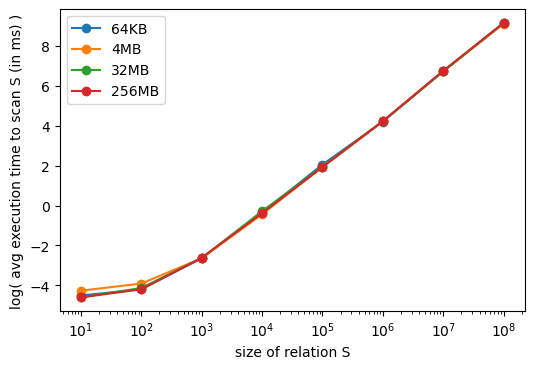
\includegraphics[width=5cm, height=4cm]{3b-1.png}
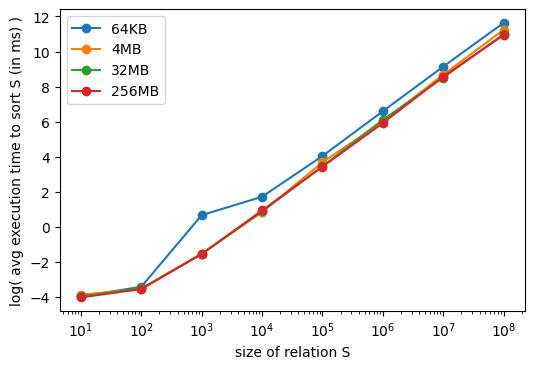
\includegraphics[width=5cm, height=4cm]{3b-2.png}
\caption{Summary of 3(b). Left panel: avgerage execution time to scan S. Right panel: avg execution time to sort S. Vertical and horizontal axis are in  logarithmic scale.}
\end{center}
\end{figure}

\textbf{Execution time with different working memory:}
%% TABLE - 64KB
\begin{table}[H]
\begin{center}
\begin{tabular}{c|c|c}
size $n$ of relation {\tt S} & avg execution time to \textcolor{red}{scan} {\tt S} (in ms) &avg execution time to \textcolor{red}{sort} {\tt S} (in ms) \\ \hline
$10^1$&  0.011 &  0.019\\
$10^2$&  0.015 &  0.033\\
$10^3$&  0.071 &  1.960\\
$10^4$&  0.703 &  5.588\\
$10^5$&  7.803 & 57.190\\
$10^6$& 67.268 &735.341\\
$10^7$&834.039 &9355.402\\
$10^8$&9416.056&113257.111\\
\end{tabular}
\caption{Work memory = 64kB}
\end{center}
\end{table}

%% TABLE - 4MB
\begin{table}[H]
\begin{center}
\begin{tabular}{c|c|c}
size $n$ of relation {\tt S} & avg execution time to \textcolor{red}{scan} {\tt S} (in ms) &avg execution time to \textcolor{red}{sort} {\tt S} (in ms) \\ \hline
$10^1$&  0.014 &  0.021\\
$10^2$&  0.020 &  0.029\\
$10^3$&  0.071 &  0.217\\
$10^4$&  0.647 &  2.328\\
$10^5$&  6.904 & 40.048\\
$10^6$& 67.846 &408.421\\
$10^7$&842.501 &5871.563\\
$10^8$&9068.983&76482.252\\
\end{tabular}
\caption{Work memory = 4MB}
\end{center}
\end{table}

%% TABLE - 32MB
\begin{table}[H]
\begin{center}
\begin{tabular}{c|c|c}
size $n$ of relation {\tt S} & avg execution time to \textcolor{red}{scan} {\tt S} (in ms) &avg execution time to \textcolor{red}{sort} {\tt S} (in ms) \\ \hline
$10^1$&  0.010 &  0.019\\
$10^2$&  0.016 &  0.030\\
$10^3$&  0.072 &  0.213\\
$10^4$&  0.754 &  2.435\\
$10^5$&  6.982 & 31.596\\
$10^6$& 68.361 &449.457\\
$10^7$&841.679 &4985.135\\
$10^8$&9398.008&59461.610\\
\end{tabular}
\caption{Work memory = 32MB}
\end{center}
\end{table}

%% TABLE - 256MB
\begin{table}[H]
\begin{center}
\begin{tabular}{c|c|c}
size $n$ of relation {\tt S} & avg execution time to \textcolor{red}{scan} {\tt S} (in ms) &avg execution time to \textcolor{red}{sort} {\tt S} (in ms) \\ \hline
$10^1$&  0.010 &  0.018\\
$10^2$&  0.015 &  0.029\\
$10^3$&  0.073 &  0.215\\
$10^4$&  0.680 &  2.554\\
$10^5$&  6.878 & 31.088\\
$10^6$& 69.094 &374.019\\
$10^7$&857.698 &5299.657\\
$10^8$&9510.330&56507.911\\
\end{tabular}
\caption{Work memory = 256MB}
\end{center}
\end{table}

\subsubsection*{(c)}
In query plan, either quick sort or external merge sort is used depending on the size of $S$. The time to create index increases sharply. However, with index, the execution time for range query improves to some extend.Compared with simulation in 3(b) with the same working memory, the execution time with index is less when the size of relation is no greater than $10^7$.
\begin{table}[H]
\begin{center}
\begin{tabular}{c|c|c}
size $n$ of relation {\tt S} & avg execution time to create index indexedS &avg execution time for range query (in ms) \\ \hline
$10^1$&1.039  &        0.103\\
$10^2$&1.232  &        0.028\\
$10^3$&4.998  &        0.139\\
$10^4$&34.141 &        1.206\\
$10^5$&437.413 &       13.173\\
$10^6$&4621.796 &      132.350\\
$10^7$&99253.394 &     2337.960\\
$10^8$&7044649.479 &  1056646.735\\
\end{tabular}
\caption{Work memory = 4MB; Range query with index}
\end{center}
\end{table}


\subsection*{4.}
%% This is the answer to Problem 4.
\redbullet\ %\textcolor{red}{\bf Practice problem-not graded}.
Typically, the {\tt makeS} function returns a bag instead of a set.   In the problems in this section, you are to conduct
experiments to measure the execution times to eliminate duplicates.   

\begin{enumerate}
\item \label{duplicateDistinct} 
Write a SQL query that uses the \blue{\tt DISTINCT} clause to eliminate duplicates in {\tt S} and 
report you results in a table such as that in Problem 3.

\begin{center}
\begin{tabular}{c|c|c}
size $n$ of relation {\tt S} & avg execution time to \textcolor{red}{scan} {\tt S} (in ms) &avg execution time to \textcolor{red}{sort} {\tt S} (in ms) \\ \hline
$10^1$ & 0.046 & 0.067 \\
$10^2$ & 0.091 & 0.124 \\
$10^3$ & 0.595 & 0.947 \\
$10^4$ & 5.557 & 8.302 \\
$10^5$ & 94.951 & 156.484 \\
$10^6$ & 1506.690 & 2118.828 \\
$10^7$ & 16514.796 & 25351.566 \\
\end{tabular}
\end{center}

\item \label{duplicateGroupBy}  Write a SQL query that uses the \blue{\tt GROUP BY} clause to eliminate duplicates in {\tt S} and 
report you results in a table such as that in Problem 3.

\begin{center}
\begin{tabular}{c|c|c}
size $n$ of relation {\tt S} & avg execution time to \textcolor{red}{scan} {\tt S} (in ms) &avg execution time to \textcolor{red}{sort} {\tt S} (in ms) \\ \hline
$10^1$ & 0.054 & 0.068 \\
$10^2$ & 0.138 & 0.152 \\
$10^3$ & 0.900 & 1.235 \\
$10^4$ & 6.332 & 11.097 \\
$10^5$ & 89.268 & 143.469 \\
$10^6$ & 1183.692 & 1007.643 \\
$10^7$ & 12917.292 & 12713.808 \\
\end{tabular}
\end{center}

\item Compare and contrast the results you have obtained in problems~\ref{duplicateDistinct} and \ref{duplicateGroupBy}.
Again, consider using \blue{\tt explain analyze} to look at query plans.

When the data size is small, the query plan of using distinct without ordering is HashAggregate (group key is x), the query plan of using distinct with ordering is Sort (quicksort here) and HashAggregate, the query plan of using group by without ordering is HashAggregate (group key is x), and the query plan of using group by with ordering is Sort (quicksort) and HashAggregate. We find that the fastest version is using distinct without ordering, followed by using distinct with ordering, using group by without ordering, and using group by with ordering.

When the data size becomes large, external merge is utilized for sorting. Moreover, the group by clause begins to use partitions (HashAggregate with buckets for hashing and GroupAggregate with partitions for sorting). We can see that the group by clauses run faster, and the version with ordering is the fastest.

\end{enumerate}




\subsection*{7.}

\[ M \leq \frac{blocksize}{\mid blockaddress \mid + \mid key \mid } =  \frac{8192}{18} = 455\]

\[  227 = \frac{M}{2}   \leq r \leq M \]


let height \[ h = log_\frac{M}{2} \frac{2N}{r}   \]

\[ N = 10^{10} \]
\begin{itemize}
  \item 7 (a) \newline

  \[ T_{min} =   t  *  log_{2} M  *   log_{\frac{M}{2}} N + t * log_{2} r\]

  \[ T_{min} =   679 ms\]


  \item 7(b)
  
    \[ h = log_\frac{M}{2} \frac{2N}{r} =  log_\frac{455}{2} \frac{2*10^{10}}{227} = 3.37 \]

    \[ t = 45 ms\]
  
  \item 7(c)
As for the first 2 levels    \[ \frac{(10 + 8 ) * 455 * 455 }{1024^2} = 3.4 MB\]
As for the first 3 levels    \[ \frac{(10 + 8 ) * 455 * 455^2 }{1024^2} = 1.5GB\]

Main memory requires to store one level of B+ tree during the recursive progress of determining if a record key exists. After a level is scanned, the memory of the level can be discard, and then the corresponding block of the next level is stored to the main memory.\\
If a key is inserted, it is probable to split a block and add a key into the block of the previous level. This process may execute recursively. Therefore, at least 2 levels of B+ tree must be stored in the main memory.
  
\end{itemize}

\subsection*{8.}

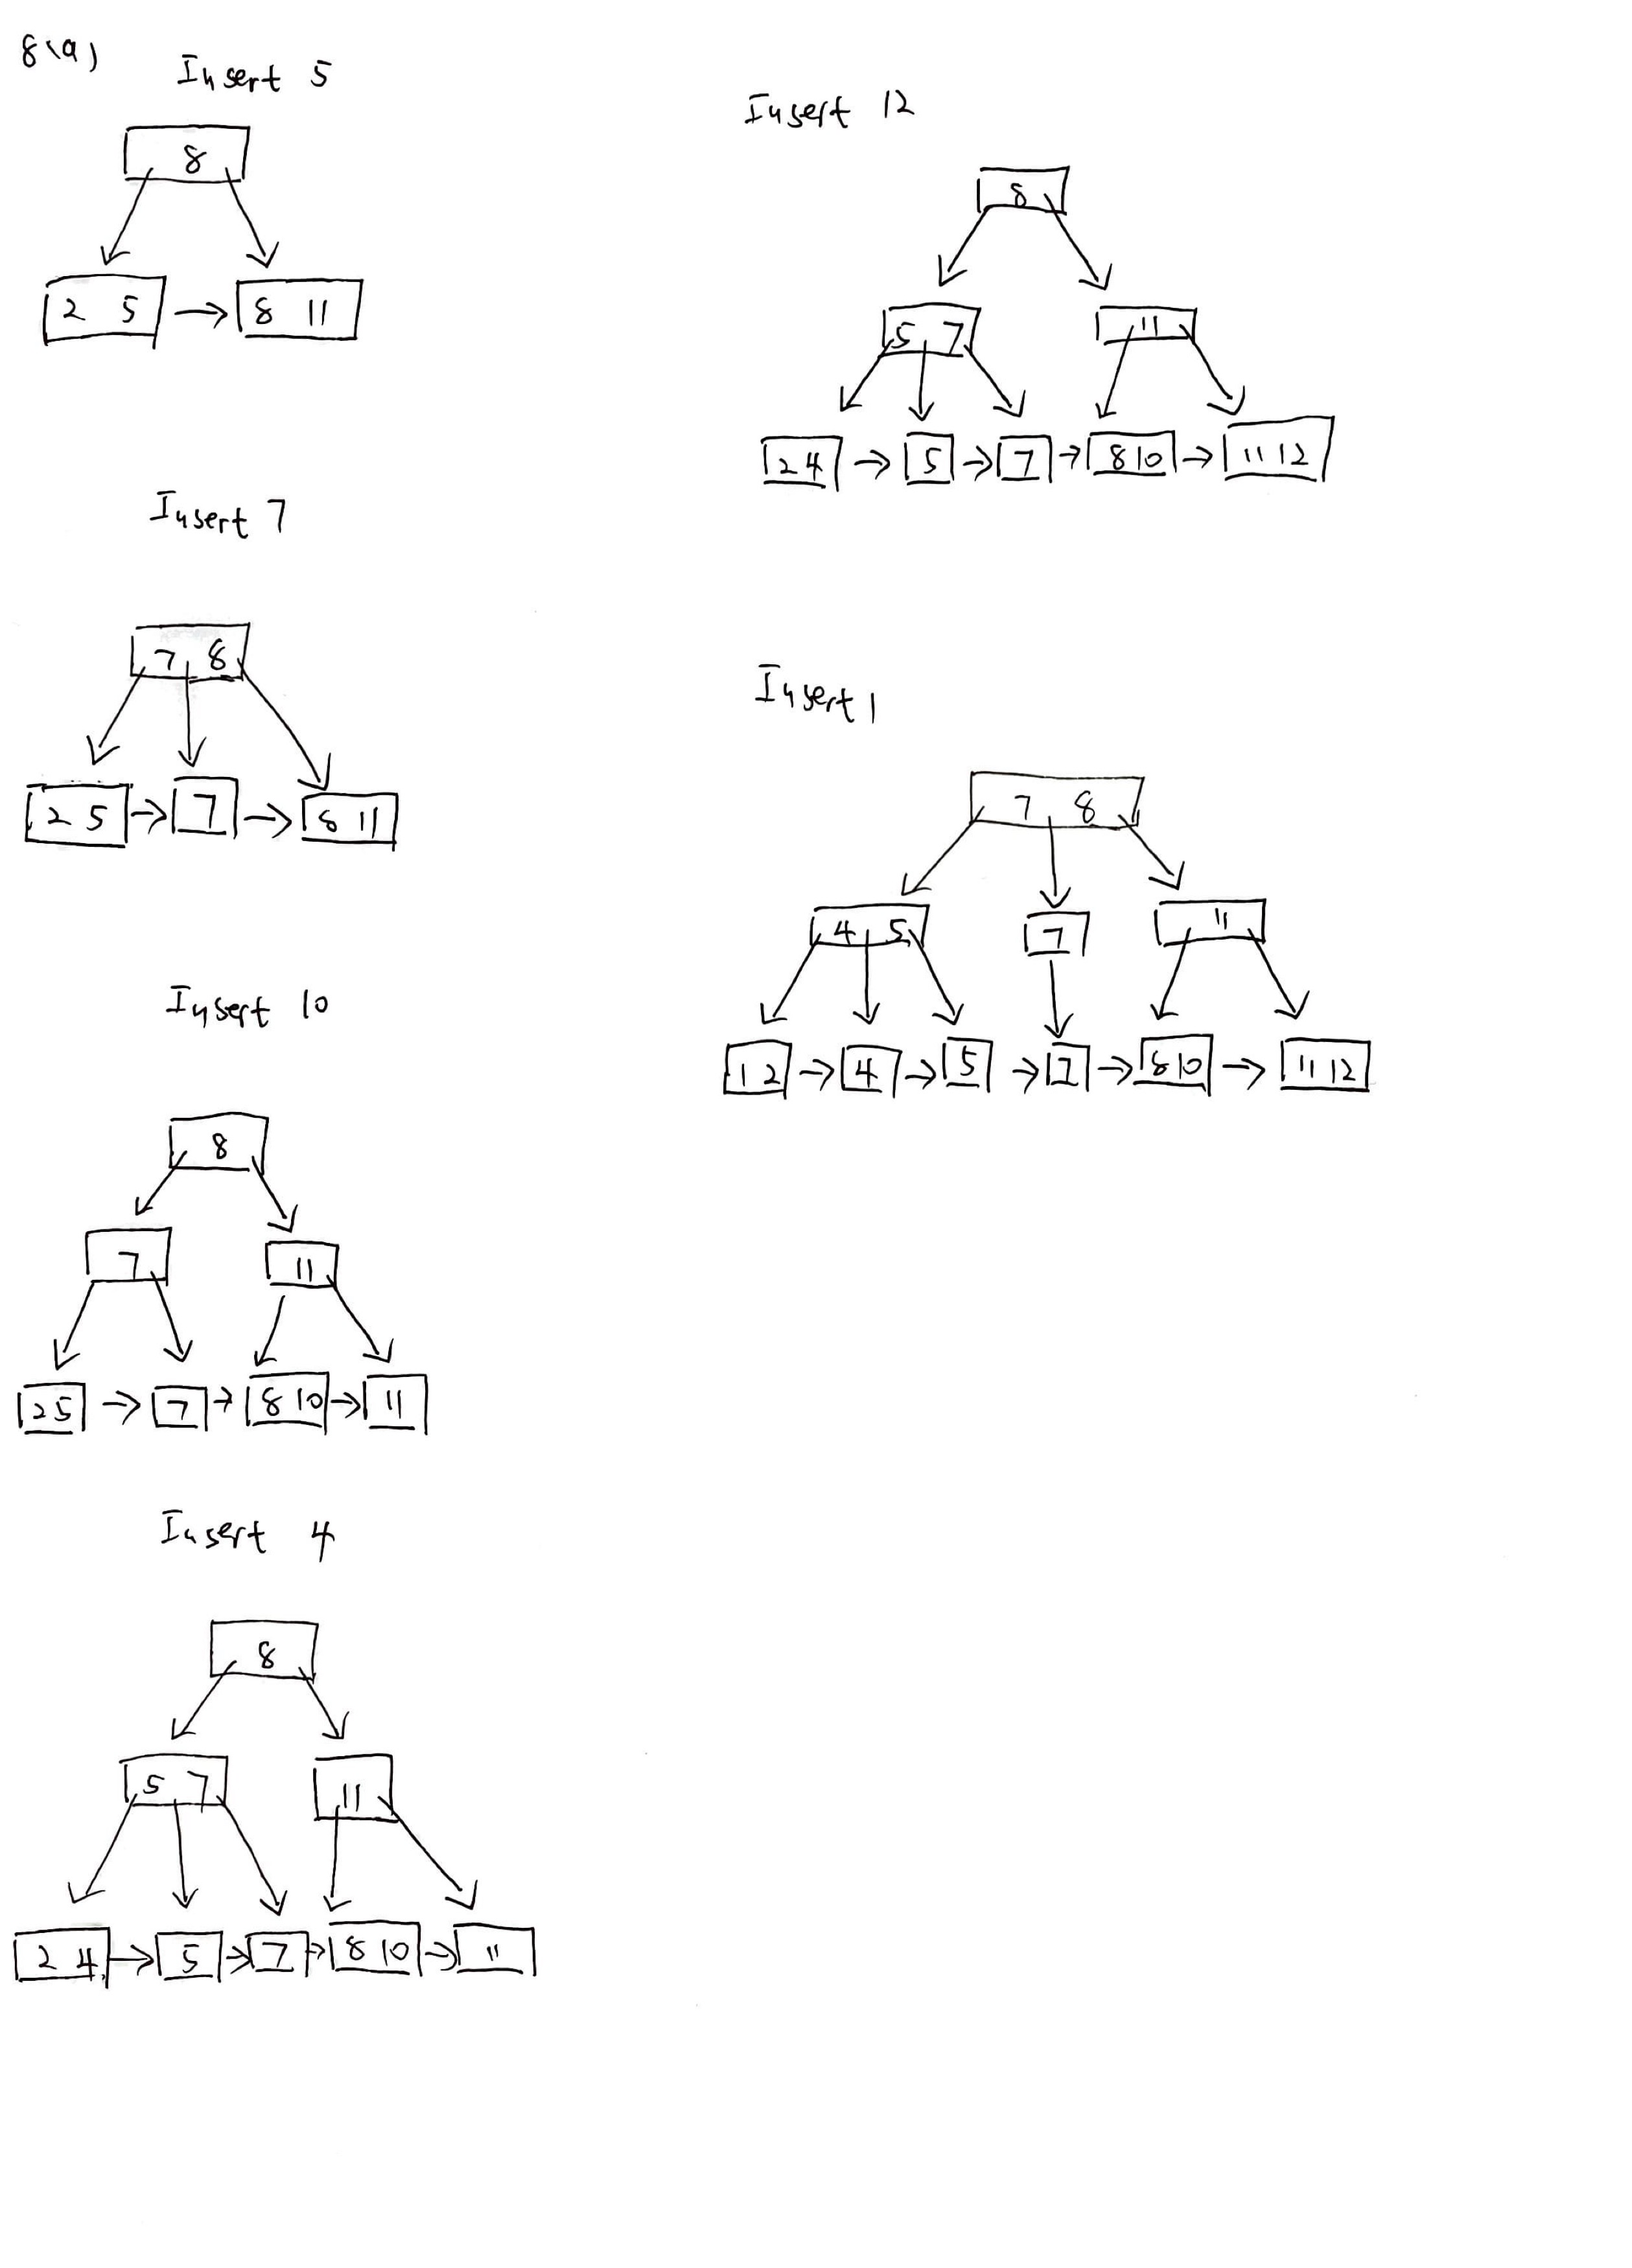
\includegraphics[width=15cm, height=20cm]{8_a}

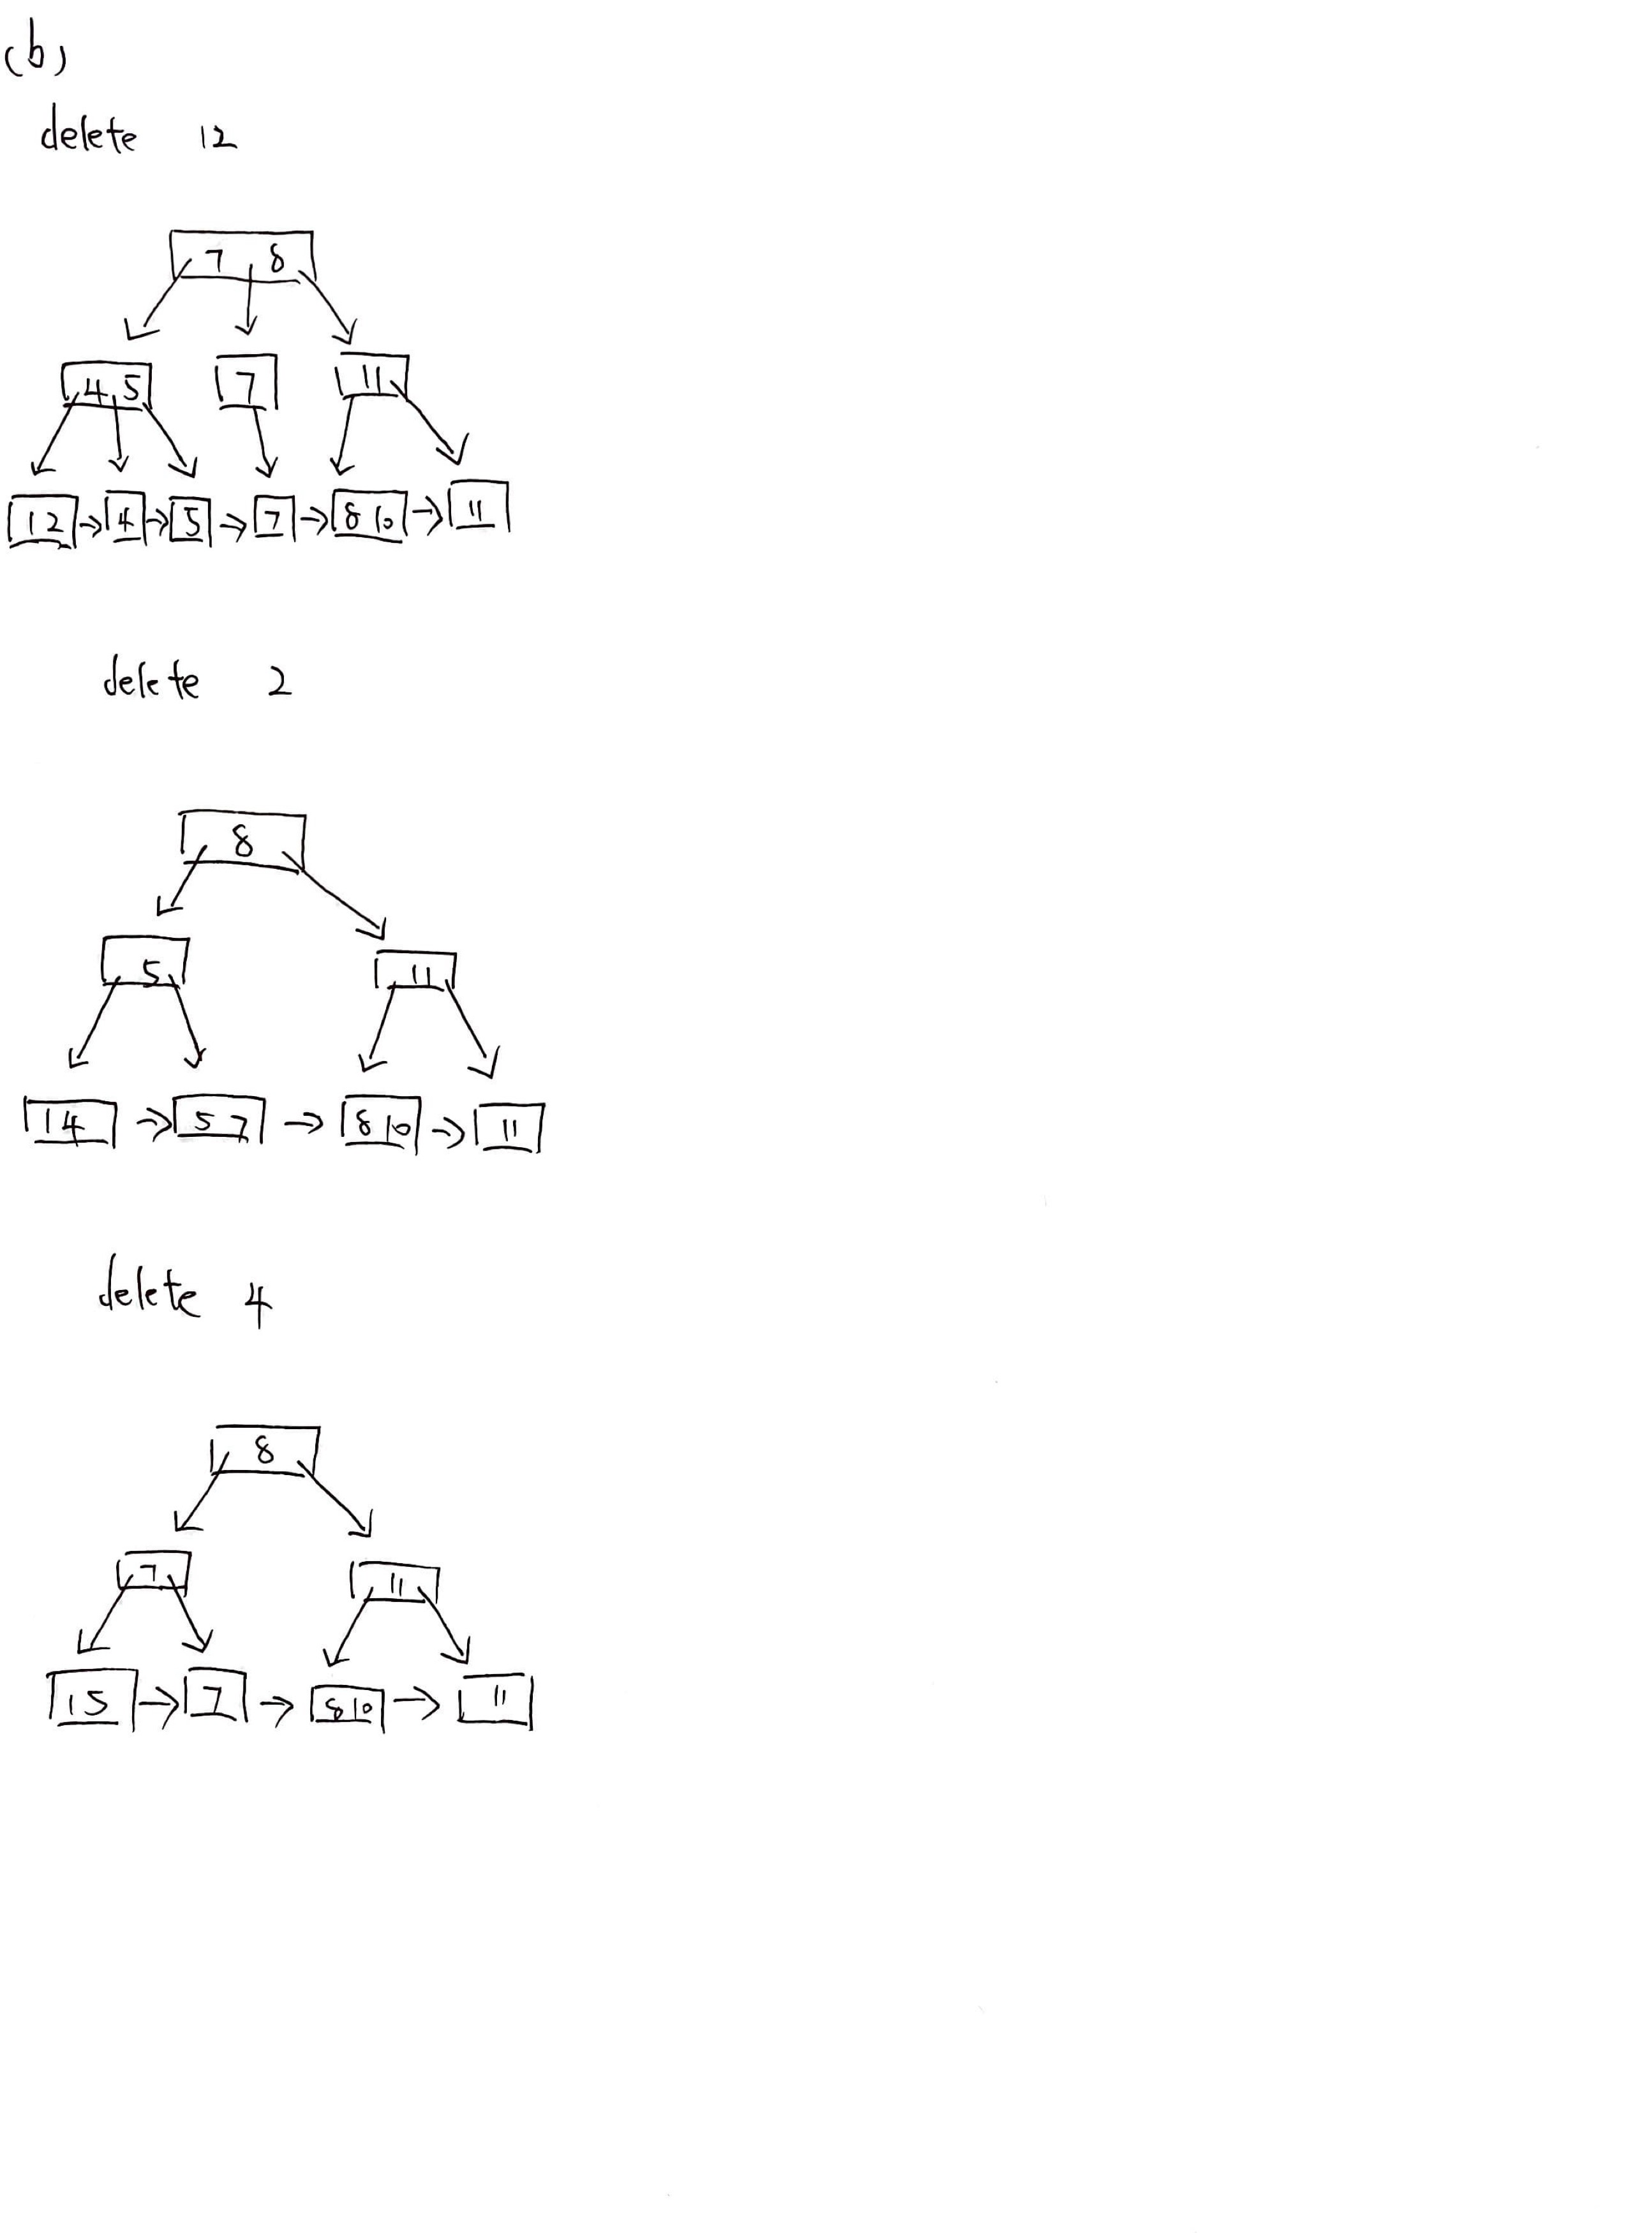
\includegraphics[width=15cm, height=20cm]{8_b}

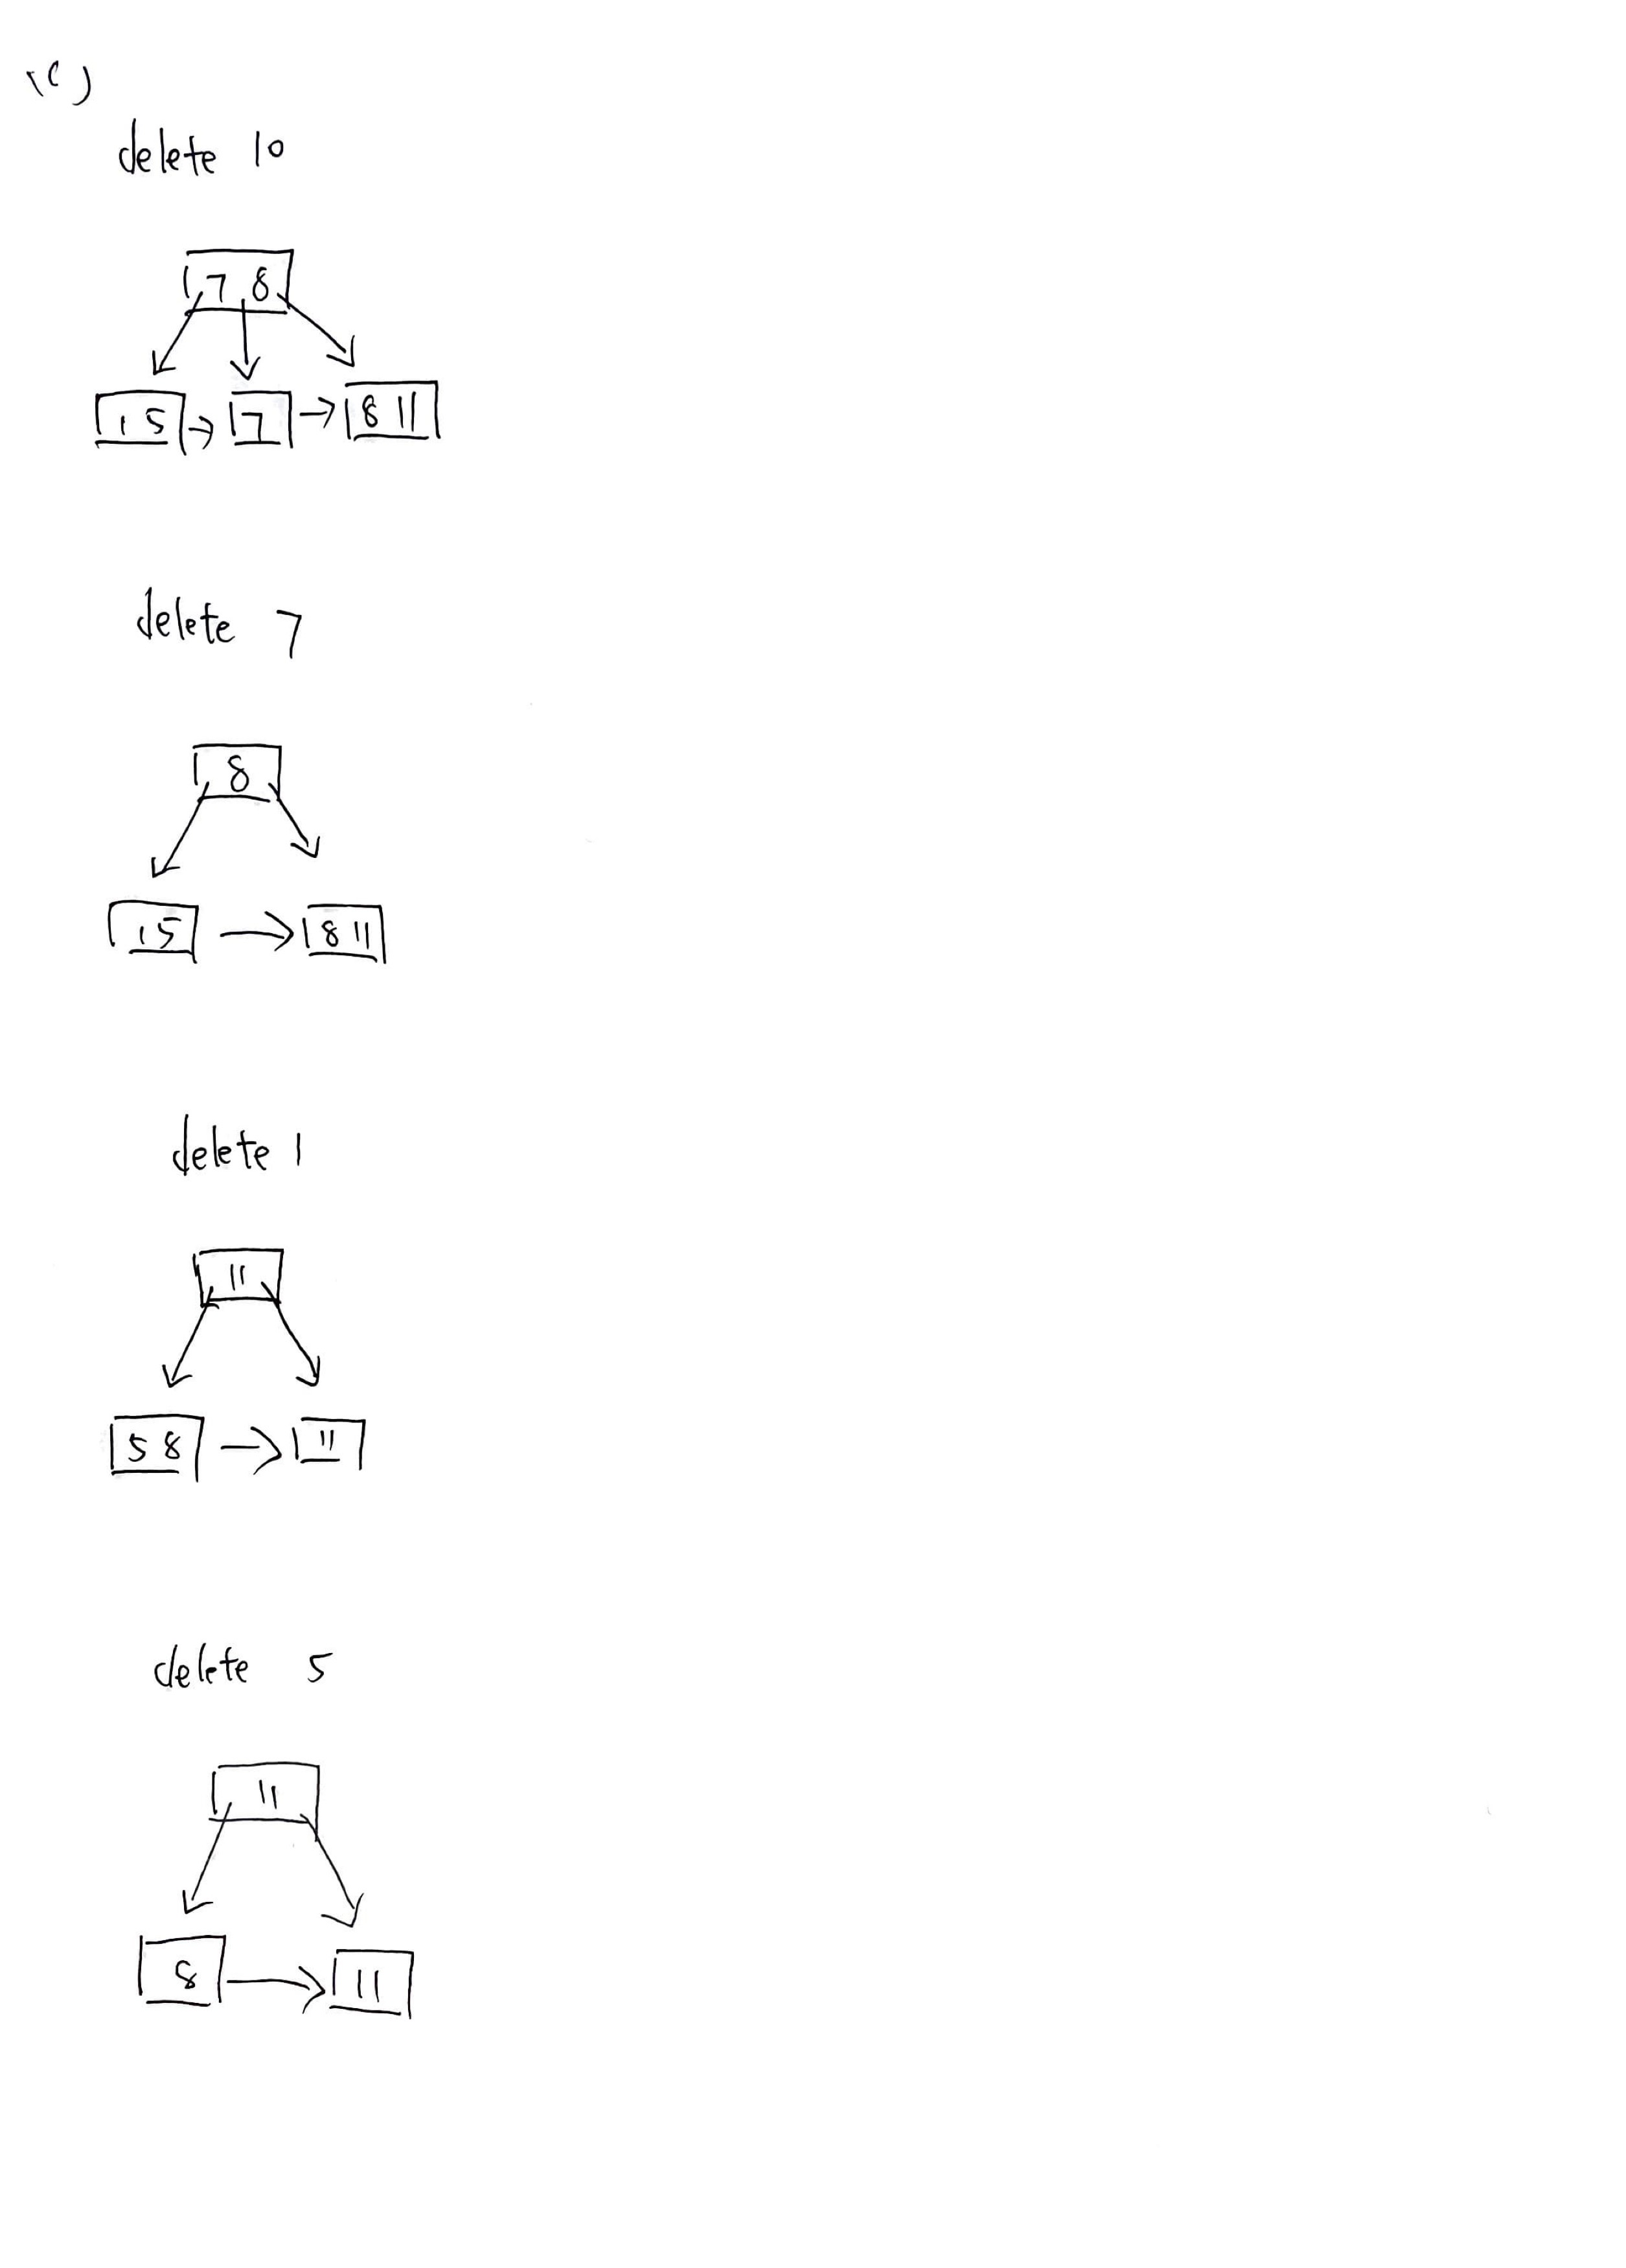
\includegraphics[width=15cm, height=20cm]{8_c}

\subsection*{9.}
\begin{figure}[h]
        \centering
        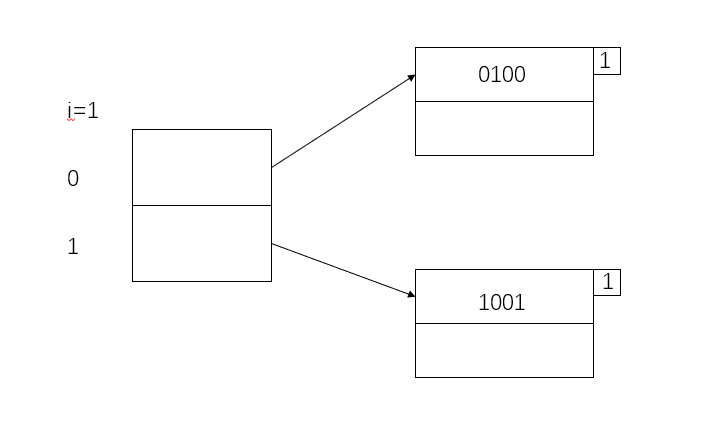
\includegraphics[height = 1.5in, width = 3in]{figure/9a1.png}
        \caption{a1}
    \end{figure}
\bigskip


\begin{figure}[h]
        \centering
        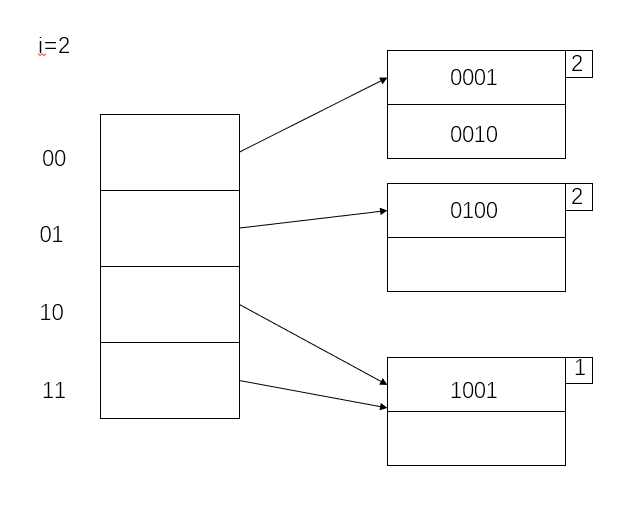
\includegraphics[height = 1.5in, width = 3in]{figure/9a2.png}
        \caption{9-a2}
    \end{figure}
\bigskip



\begin{figure}[h]
        \centering
        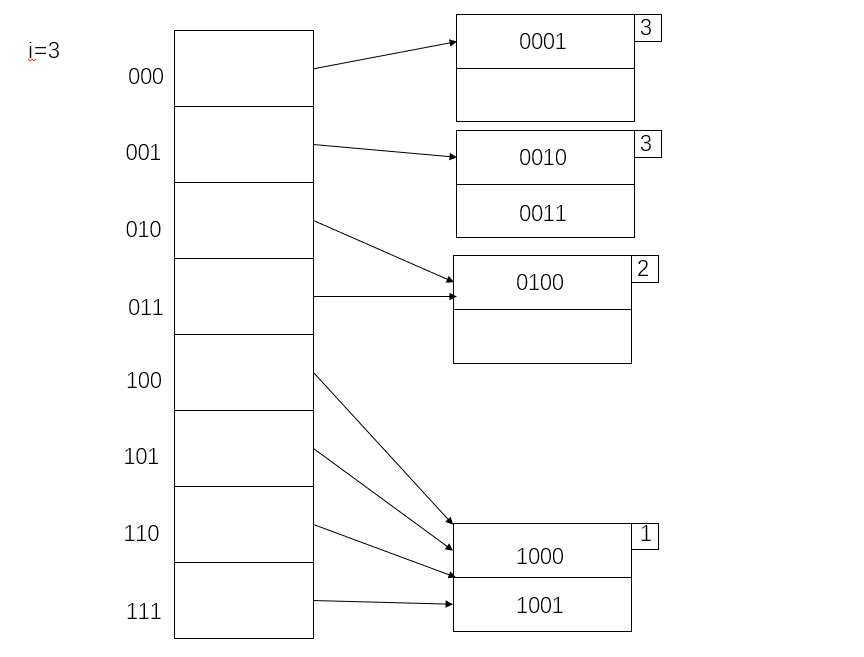
\includegraphics[height = 1.5in, width = 3in]{figure/9a3.png}
        \caption{9-a3}
    \end{figure}
\bigskip

\begin{figure}[h]
        \centering
        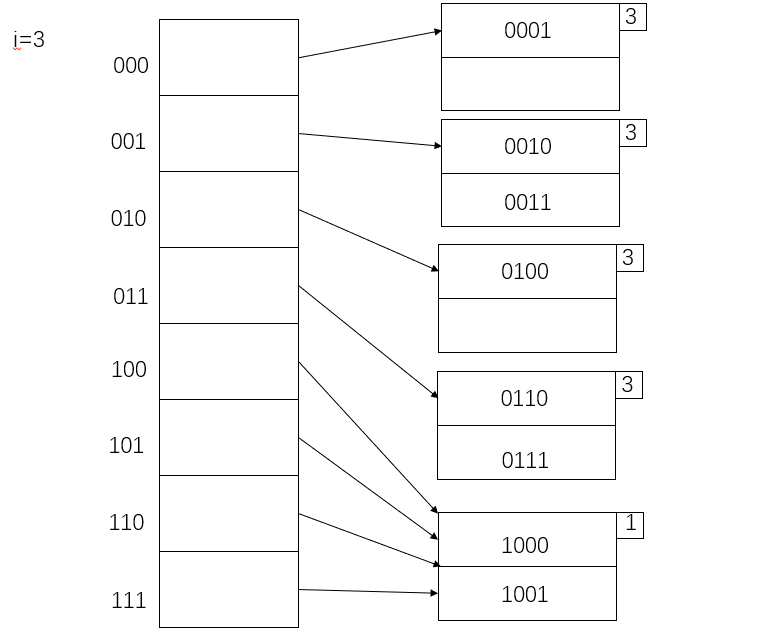
\includegraphics[height = 1.5in, width = 3in]{figure/9a4.png}
        \caption{9-a4}
    \end{figure}
\bigskip

\begin{figure}[h]
        \centering
        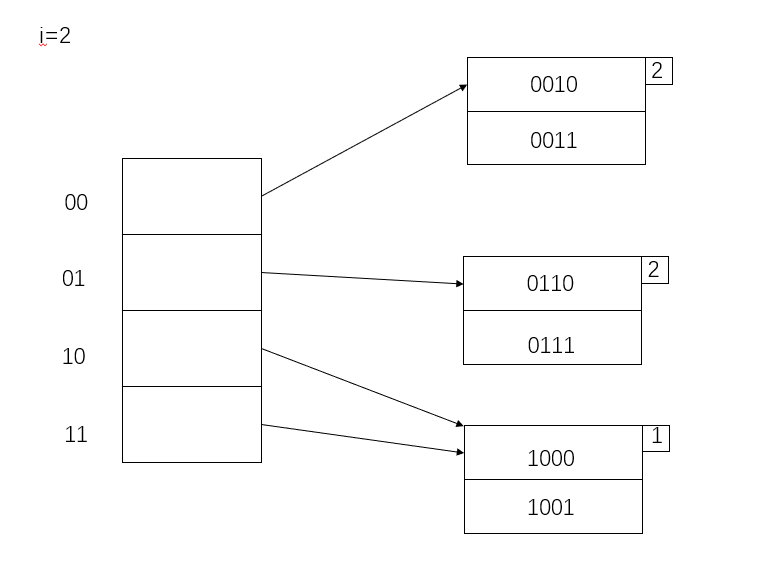
\includegraphics[height = 1.5in, width = 3in]{figure/9b1.png}
        \caption{9-b1}
    \end{figure}
\bigskip


\begin{figure}[h]
        \centering
        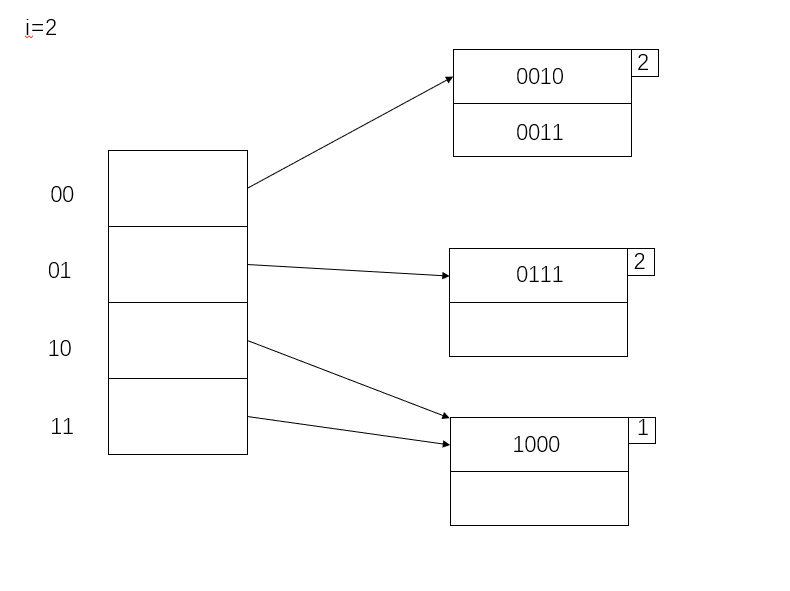
\includegraphics[height = 1.5in, width = 3in]{figure/9b2.png}
        \caption{9-b2}
    \end{figure}
\bigskip
\begin{figure}[h]
        \centering
        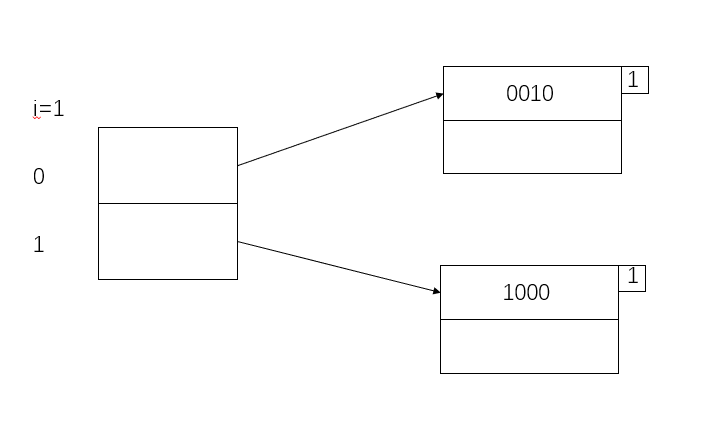
\includegraphics[height = 1.5in, width = 3in]{figure/9b3.png}
        \caption{9-b3}
    \end{figure}
\bigskip
\clearpage

\subsection*{10.}
In this task, an index with $B^+$ tree is generate. We compare the performance with/without index for a query. Relations are generated with \texttt{GeneratepersonSkillRelation} in small, medium and large size. The approximate size is shown in the first column of table below. \\
With small size, the index will not improve execution time; with medium size, indexing decreases time for query; with large size, query without index outperforms the other case again. For the third case, it may be a random case and could be changed with multiple independent runs.
\begin{table}[H]
\begin{center}
\begin{tabular}{c|c|c}
size of relation & execution time (in ms)without index& execution time (in ms) with index \\ \hline
$\sim 10^2$ & 0.042 & 0.043 \\
$\sim 10^4$ & 2.582 & 0.886 \\
$\sim 10^6$ &280.602& 375.876 \\
\end{tabular}
\end{center}
\end{table}


\subsection*{11.}
%% This is Problem 11
\redbullet\  Create an appropriate index on the {\tt worksFor} relation that speedups the range query
\begin{alltt}\textcolor{blue}{
select pid
from   worksFor
where  \textcolor{red}{s1} <= salary and salary <= \textcolor{red}{s2};}
\end{alltt}
Here \textcolor{red}{s1} and \textcolor{red}{s2} are two salaries with $\text{s1} \leq \text{s2}$.

Illustrate and discuss this speedup by finding the execution times for this query for 3 different
but sufficiently large sizes of the {\tt worksFor} relation.

\begin{center}
\title{results on table with $10^6$ rows}
\\ \hspace*{\fill} \\
\begin{tabular}{c|c|c}
\hline
range scale & execution time \textcolor{red}{without} index (in ms) & execution time \textcolor{red}{with} index (in ms) \\ \hline
small & 92.075 & 1.767 \\
intermediate & 124.687 & 74.501 \\
maximum & 187.037 & 188.379 \\
\hline
\end{tabular}
\end{center}

\begin{center}
\title{results on table with $10^7$ rows}
\\ \hspace*{\fill} \\
\begin{tabular}{c|c|c}
\hline
range scale & execution time \textcolor{red}{without} index (in ms) & execution time \textcolor{red}{with} index (in ms) \\ \hline
small & 871.667 & 1.535 \\
intermediate & 1545.504 & 1667.705 \\
maximum & 3015.498 & 3162.538 \\
\hline
\end{tabular}
\end{center}

\begin{center}
\title{results on table with $10^8$ rows}
\\ \hspace*{\fill} \\
\begin{tabular}{c|c|c}
\hline
range scale & execution time \textcolor{red}{without} index (in ms) & execution time \textcolor{red}{with} index (in ms) \\ \hline
small & 618.999 & 10.385 \\
intermediate & 1461.404 & 1556.531 \\
maximum & 3155.947 & 3368.145 \\
\hline
\end{tabular}
\end{center}

We used Btree to construct index. From the execution time we can find that: 1) using index can speed up the query execution. 2) With a large range, the speedup becomes not obvious.

This is reasonable. Because when we use the maximum range, what Btree does is going down to a leaf node and then follow the links between the leaf nodes to all the other nodes, which is about the same time as scaning the table.
\subsection*{12.}

We use build Hash index for pid. Then run experiments in three large enough datasets($10^5$,$10^6$ and $10^7$) several times and calculate the average execution time. The results are as following: 
\begin{center}
\title{results on table.}
\\ \hspace*{\fill} \\
\begin{tabular}{c|c|c}
\hline
dataset scale & execution time \textcolor{red}{without} index (in ms) & execution time \textcolor{red}{with} index (in ms) \\ \hline
$10^5$ rows &  17.540 & 0.057 \\
$10^6$ rows & 122.217 & 0.066 \\
$10^7$ rows & 483.346 & 0.164 \\
\hline
\end{tabular}
\end{center}

We can see that Hash index cut the execution time in different large datasets obviously.

\subsection*{13.}

\begin{center}
\title{results on table person with $10^4$ rows, table personSkill $2*10^4$ but actually $16453$ rows}
\\ \hspace*{\fill} \\
\begin{tabular}{c|c|c}

\hline
[not] in & execution time without index (in ms) & execution time with index (in ms) \\ \hline
in & 5.989  & 4.065 \\
not in & 3.764 & 4.065 \\

\hline
\end{tabular}
\end{center}



\begin{center}
\title{results on table person with $10^5$ rows, table personSkill $3*10^5$ but actually $225857$ rows}
\\ \hspace*{\fill} \\
\begin{tabular}{c|c|c}
\hline
[not] in & execution time without index (in ms) & execution time with index (in ms) \\ \hline
in & 56.03  & 59.332 \\
not in & 47.204 & 46.696 \\

\hline
\end{tabular}
\end{center}



\begin{center}
\title{results on table person with $10^6$ rows, table personSkill $3*10^6$ but actually $498725$ rows}
\\ \hspace*{\fill} \\
\begin{tabular}{c|c|c}
\hline
[not] in & execution time without index (in ms) & execution time with index (in ms) \\ \hline
in & 72.099  & 78.412 \\
not in & 369.249 & 373.367 \\

\hline
\end{tabular}
\end{center}
Person \textbf{pid} is generated with fixed certain row number. However, the personSkill are generated with random() method and there are tremendous numbers of duplicates. As for this case, index on primary key does \textbf{not} have a significant improvement opon speeding.
\subsection*{14.}
\end{document}
